\documentclass{article}
\usepackage[left=2cm, right=2cm, top=2cm]{geometry}
\usepackage[utf8]{inputenc}
\usepackage{amsthm,amsmath,amsfonts,amssymb,graphicx}
\usepackage{algorithm}
\usepackage{caption}
\usepackage{subcaption}
\usepackage[noend]{algpseudocode}

\title{Segmentation of Heatmaps}
%\author{T.L. Grobler}

\begin{document}
\maketitle
\begin{abstract}
\end{abstract}
Most often, when we first inspect a dataset containing the temporal-spatial coordinates of multiple objects (i.e. the movements of say humans, animals or vessels) we would create a heat-map (grid data onto a two-dimensional grid) so that we can build some intuition (gather information) about the data.
This intuition can then be used to further analyze the original data. This intuition can be built up by extracting the following information from a heat-map: the high volume 
routes and regions (this is not meant to be an exhaustive list). In this paper, we present an automatic heat-map segmentation algorithm which will allow us to accomplish exactly this.
In this paper we focus on Automatic Identification System (AIS) data, which can be used to help track the movement of ships at sea. The pseudo-code of the proposed segmentation algorithm is given in Algorithm 1. 
\begin{algorithm}
 \caption{AIS Polygon Heat-map Segmentation Algorithm}\label{euclid}
 \begin{algorithmic}[1]
 \Procedure{polygonSegmentation}{heatmap,coastlinemask,landmask}
 \State $\textrm{heatmap} \gets \log(\textrm{heatmap}+1)$
 \Comment{emphasizes the linear tracks}
 \State $\textrm{copy} \gets \textrm{heatmap}$
 \Comment{store a copy of original}
 \State $\textrm{heatmap} \gets \textrm{maskCoastline(heatmap,coastlinemask)}$
 \Comment{mask coastline}
 \State $\textrm{heatmap} \gets \textrm{heatmap - medianFilter(heatmap)}$ 
 \Comment{emphasizes the linear tracks}
 \State $\textrm{heatmap} \gets \textrm{otsuThreshold(heatmap)}$
 \Comment{binary segmentation}
 \State $\textrm{heatmap} \gets \textrm{binaryOpening(heatmap)}$
 \Comment{clears the noisy region}
 \State $\textrm{lines} \gets \textrm{houghTransform(heeatmap)}$
 \Comment{extract lines from image}
 \State $\textrm{polygons} \gets \textrm{polygonize(lines,coastlinemask,landmask)}$
 \Comment{polygonize}
 \For{polygon in polygons}
     \State $\textrm{heatmap[polygon]} \gets \textrm{average(copy[polygon])}$ 
 \EndFor
 \State $\textrm{heatmap[coastlinemask]} \gets \textrm{average(copy[polygon])}$
 \State $\textrm{heatmap[landmask]} \gets 0$
 \Comment{segmentation}
 \State plot(heatmap)
 
 % \State $\textit{stringlen} \gets \text{length of }\textit{string}$
% \State $i \gets \textit{patlen}$
% %\BState \emph{top}:
% \If {$i > \textit{stringlen}$} \Return false
% \EndIf
% \State $j \gets \textit{patlen}$
% %\BState \emph{loop}:
% \If {$\textit{string}(i) = \textit{path}(j)$}
% \State $j \gets j-1$.
% \State $i \gets i-1$.
% \State \textbf{goto} \emph{loop}.
% \State \textbf{close};
% \EndIf
% \State $i \gets i+\max(\textit{delta}_1(\textit{string}(i)),\textit{delta}_2(j))$.
% \State \textbf{goto} \emph{top}.
 \EndProcedure
 \end{algorithmic}
 \end{algorithm}
The first step in the algorithm is to take the elment-wise logarithm of the heatmap. This visually emphasises the high volume routes found within the heatmap. We then 
create a binary image. To achieve this we first filter the logged heatmap. We make use of a median filter as it is well known for its ability to detect outliers. We then threshold (we used Otsu thresholding) the  
filtered heatmap. To clean the binary heatmap (we obtained by applying thresholding) we make use of morphological opening (which is used to remove noise from the foreground).
We then use the Hough Transform to extract the longer lines from the opened binary heatmap. We then polygonize the image using the extracted lines. We can then 
segment the image into different regions using the aforementioned derived polygons. The result of applying the above algorithm to AIS data is depicted in Figure!\ref{}.


There are some short commings in the algorithm. The Hough-Transform struggles to detect all 
the lines. It especially struggles with short and closely spaced parallel lines. Some of the line segments should 
 
 The logarithm of the heatmap is computed. We then  

\begin{figure}[ht] 
  \begin{subfigure}[b]{0.5\linewidth}
    \centering
    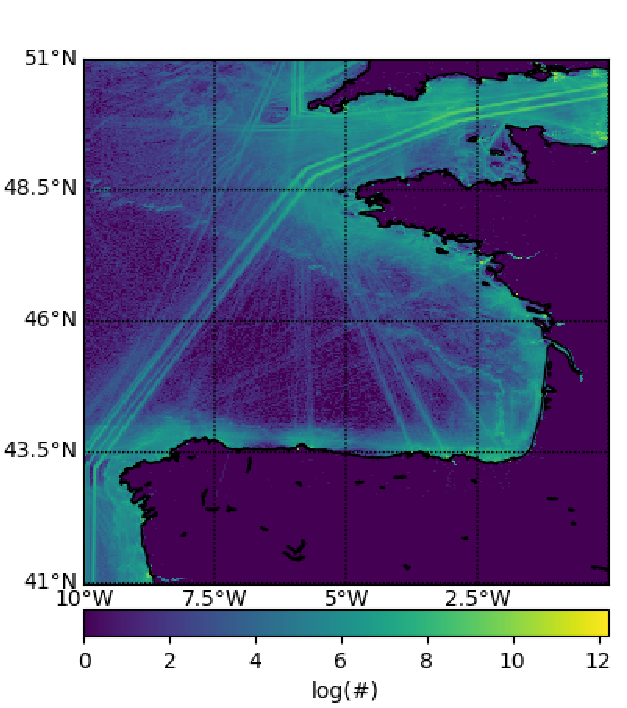
\includegraphics[width=0.8\linewidth]{CELTICcrop.pdf} 
    \caption{Logarithm applied} 
    \label{fig7:a} 
    \vspace{4ex}
  \end{subfigure}%% 
  \begin{subfigure}[b]{0.5\linewidth}
    \centering
    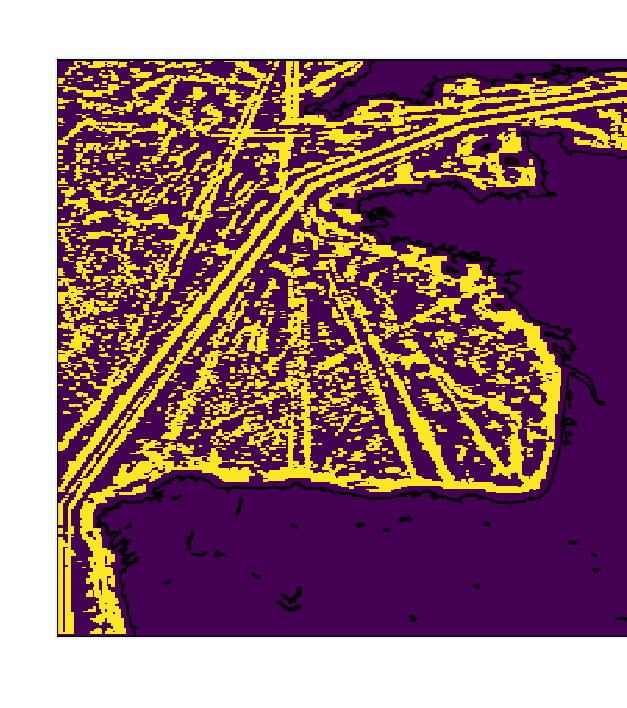
\includegraphics[width=0.8\textwidth]{CELTICopened-crop.pdf} 
    \caption{Binary segmented image} 
    \label{fig7:b} 
    \vspace{4ex}
  \end{subfigure} 
  \begin{subfigure}[b]{0.5\linewidth}
    \centering
    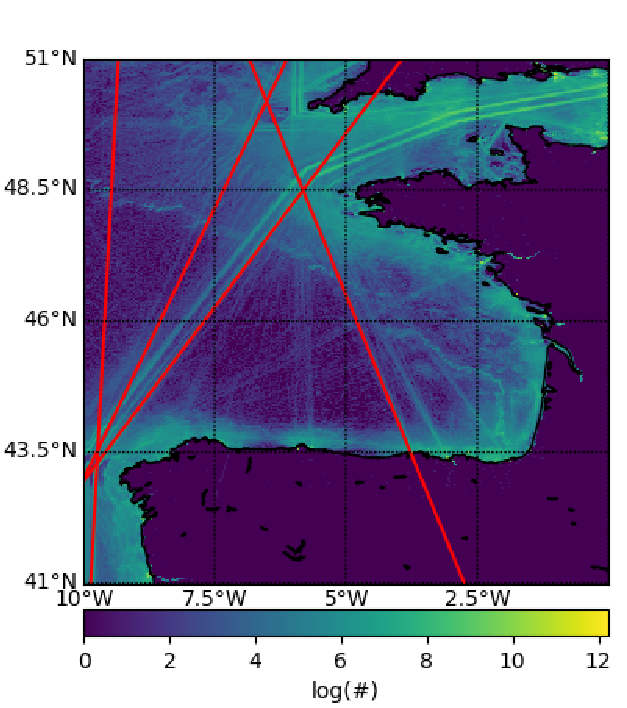
\includegraphics[width=0.8\textwidth]{CELTIClines-crop.pdf} 
    \caption{Hough Transform} 
    \label{fig7:c} 
  \end{subfigure}%%
  \begin{subfigure}[b]{0.5\linewidth}
    \centering
    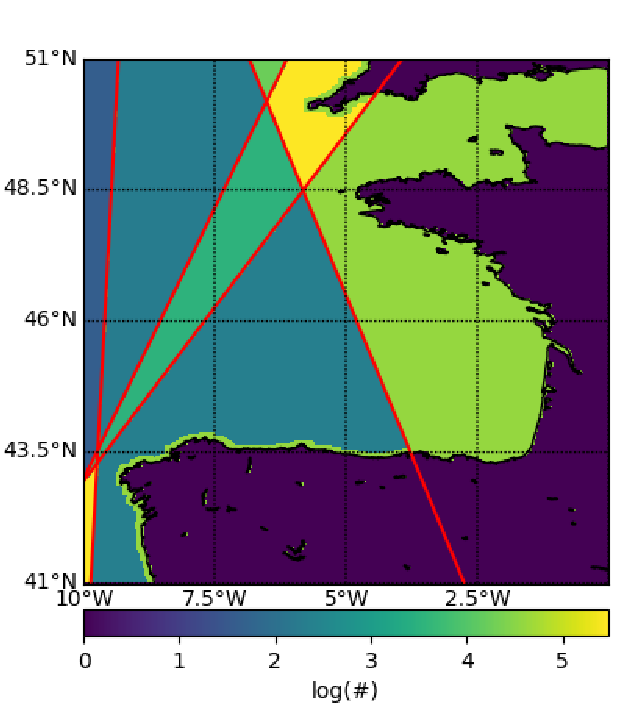
\includegraphics[width=0.8\textwidth]{CELTICsegmented-crop.pdf} 
    \caption{Segmented image} 
    \label{fig7:d} 
  \end{subfigure} 
  \caption{A heatmap of AIS ship positions within the Celtic sea, the Channel and the Bay of Biscay (France) [Longitude between $-10^{\circ}$ and $0^{\circ}$ and Latitude between $45^{\circ}$ and $51^{\circ}$]. The above subfigures were generated by applying the segmentation algorithm depicted in Algorithm 1 to an existing heatmap of the region. The top left image was optained after the logarithm of the original heatmap was taken (element-wise). The top right image 
  was obtained by applying binary thresholding and morphological opening to a filtered variant of the top left heat map. The right bottom heatmap depicts the lines we were able to extract 
  from the top right image using the Hough Transform. The bottom right image contains the final segmented heat map. Notice that the coastline is segmented separately.}
  \label{fig7} 
\end{figure}

the first thing we do is to create a heatmap of our collected data, this is to provide us with some visualization 

This document outlines a possible approach to proving that the gain solutions $\boldsymbol{g}$ can not contain a zero element. This simple idea is turning
out to be a bit harder to prove than I wish it was (maybe there is a simpler way, that I am missing). The paper is unfortunately not rigorous enough without such a proof. Altough I do believe we should submit without
this proof and try to work it into the next paper. The entire derivation works, except if $g_p = 0$ (which is exceptable ``colateral damage'' according to me). The idea is
to use the Perron-Frobenius theorem extended to complex matrices \cite{Noutsos2012}. This is a very new theorem and was derived in 2012. 



\end{document}
